
\subsection{Implementació del backend d’anàlisi}

El \textit{backend} d’anàlisi s’ha implementat com un servei local independent encarregat de concentrar la lògica que no resultava convenient executar dins del Snap. En les primeres versions del prototip, aquest component tenia una estructura simple, suficient per validar el flux inicial entre MetaMask, el Snap, el backend i Ollama. 

A mesura que el sistema va incorporar noves funcionalitats, com la normalització de transaccions, la descodificació de \textit{calldata}, el motor de regles, la persistència local i la consulta de fonts de context, es va fer necessari refactoritzar el \textit{backend} en mòduls més específics. Aquesta evolució va permetre mantenir el Snap com una capa lleugera d’intercepció i presentació, mentre que el \textit{backend} passava a assumir el paper de nucli d’anàlisi del sistema.

En la versió actual del prototip, aquest servei s’executa localment al port 3000 i exposa diversos \textit{endpoints}, entre els quals destaca \texttt{/analyze}, utilitzat pel Snap per enviar les transaccions a analitzar.


\subsubsection{Estructura general del backend}

La versió actual del \textit{backend} s’organitza en diversos mòduls amb responsabilitats diferenciades. Aquesta separació facilita el manteniment del codi, redueix l’acoblament entre parts del sistema i permet ampliar el prototip amb noves fonts de context o noves regles sense modificar tota la lògica existent.

El fitxer principal, \texttt{server.js}, actua com a punt d’entrada del servei i exposa les rutes HTTP. La resta de la lògica es delega a serveis interns encarregats de normalitzar la transacció, descodificar-ne el contingut, aplicar regles de risc, gestionar la persistència local i comunicar-se amb Ollama.

La Taula~\ref{tab:backend_moduls} resumeix els principals mòduls del \textit{backend} en la versió actual del prototip.

\begin{table}[H]
\centering
\renewcommand{\arraystretch}{1.2}
\begin{tabularx}{\textwidth}{l X}
\hline
\textbf{Mòdul} & \textbf{Funció principal} \\
\hline

\texttt{server.js} & Exposa les rutes HTTP del \textit{backend}, incloent \texttt{/analyze}, \texttt{/health} i \texttt{/stats}. \\

\texttt{analyzer.js} & Orquestra el flux complet d’anàlisi, coordinant la normalització, la descodificació, les regles, la memòria local i la generació d’explicacions. \\

\texttt{normalizeTx.js} & Converteix la transacció rebuda des del Snap a una estructura interna coherent i més fàcil de processar. \\

\texttt{decoder.js} & Intenta descodificar la \textit{calldata} de funcions conegudes, com \texttt{approve(address,uint256)} o \texttt{setApprovalForAll(address,bool)}. \\

\texttt{rules.js} & Aplica el motor determinista de regles per identificar patrons de risc i generar un veredicte estructurat. \\

\texttt{database.js} & Gestiona la base de dades SQLite local, l’historial d’anàlisis, la memòria d’adreces i les adreces conegudes. \\

\texttt{ollama.js} & Gestiona la comunicació amb Ollama i recupera les explicacions generades pel model local. \\

\hline
\end{tabularx}
\caption{Responsabilitats principals dels mòduls del \textit{backend}}
\label{tab:backend_moduls}
\end{table}

Com que la implementació JavaScript s'organitza principalment mitjançant mòduls i funcions, la Figura~\ref{fig:uml-backend} utilitza una representació UML lògica. Els estereotips indiquen el paper de cada element i les operacions enumerades corresponen als punts d'entrada més rellevants del codi, sense pressuposar una jerarquia de classes que el prototip no implementa.

\begin{figure}[H]
    \centering
    \makebox[\textwidth][c]{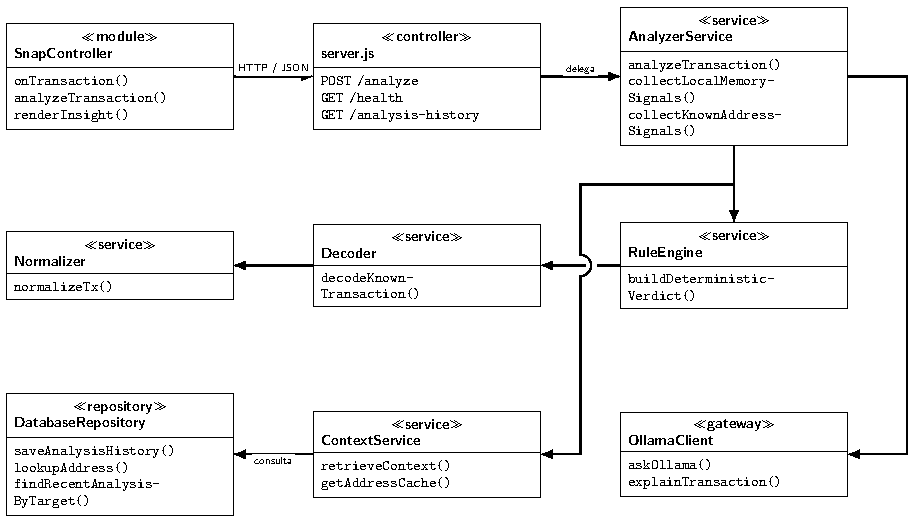
\includegraphics[width=1.04\textwidth]{diagrams/render_backend_uml.pdf}}
    \caption{Diagrama UML lògic dels mòduls, serveis i dependències principals del prototip}
    \label{fig:uml-backend}
\end{figure}

\subsubsection{Recepció de la transacció}

El punt d’entrada principal del \textit{backend} és una ruta HTTP de tipus \texttt{POST}, accessible a \texttt{http://localhost:3000/analyze}. El Snap hi envia una estructura JSON amb la informació essencial de la transacció, incloent camps com ara l’adreça d’origen, l’adreça de destinació, el valor, la \textit{calldata} i la cadena sobre la qual s’està operant. Un cop rebuda la petició, el \textit{backend} extreu aquesta informació del cos de la petició i la passa als serveis interns responsables d’analitzar-la. 

Aquest model permet desacoblar la cartera del procés d’avaluació. El Snap no necessita conèixer el detall intern de l’anàlisi, sinó únicament enviar les dades i esperar una resposta estructurada. Això fa que la comunicació entre ambdós components sigui simple i extensible.

\subsubsection{Normalització i descodificació de la petició}

Un cop rebudes les dades, el \textit{backend} normalitza la transacció a un format intern comú. Aquesta representació inclou camps com el tipus d’operació, la xarxa, l’adreça d’origen, l’adreça de destinació, el valor enviat, la \textit{calldata}, l’origen de la petició i informació derivada, com ara el selector del mètode o la identificació d’una interacció amb un contracte.

La normalització permet que la resta de mòduls treballin sobre una estructura coherent, independentment de petites diferències en el format original rebut des del Snap. D’aquesta manera, el motor d’anàlisi pot aplicar les mateixes regles sobre totes les transaccions processades.

A partir d’aquesta estructura, el sistema intenta descodificar la \textit{calldata} quan reconeix selectors de funcions conegudes. En la versió actual del prototip, el \textit{backend} identifica principalment les operacions \texttt{approve(address,uint256)} i \texttt{setApprovalForAll(address,bool)}, especialment rellevants perquè poden concedir permisos amplis sobre tokens o col·leccions NFT.

En el cas de \texttt{approve(address,uint256)}, el sistema extreu l’adreça autoritzada, representada pel camp \textit{spender}, i la quantitat concedida. En el cas de \texttt{setApprovalForAll(address,bool)}, s’obtenen l’adreça de l’operador i el valor booleà que indica si el permís global s’activa o es revoca.

Quan el selector no correspon a cap de les funcions conegudes, la transacció es manté identificada com una interacció amb un contracte no descodificada. Aquesta informació s’utilitza posteriorment pel motor de regles per aplicar un criteri més conservador.

\subsubsection{Motor de regles deterministes}

Sobre la informació normalitzada i descodificada, el \textit{backend} aplica un conjunt de regles deterministes per estimar el risc de l’operació. Aquestes regles constitueixen el mecanisme principal de classificació del sistema i produeixen un resultat estructurat que pot incloure un nivell de risc, una puntuació, una acció recomanada i un conjunt d’indicis justificatius.

En les operacions ERC20, el sistema diferencia entre tres situacions principals. Una quantitat igual a zero s’interpreta com una revocació del permís i es considera una operació de risc baix. Una aprovació amb una quantitat limitada rep igualment un tractament de risc reduït, sempre que no existeixin altres indicadors addicionals. En canvi, una aprovació equivalent a \texttt{MaxUint256}, o considerada pràcticament il·limitada, genera un nivell de risc alt i una recomanació de revisar l’operació abans de confirmar-la.

En les operacions ERC721, la crida \texttt{setApprovalForAll(operator,true)} s’interpreta com la concessió d’un permís global sobre tots els NFTs de l’usuari dins d’una col·lecció concreta. Per aquest motiu, el sistema la classifica com una operació d’alt risc. En canvi, \texttt{setApprovalForAll(operator,false)} correspon a una revocació del permís global i rep un tractament de risc baix.

Quan la transacció correspon a una interacció amb un contracte que no pot ser descodificada mitjançant els selectors implementats, el sistema pot assignar un nivell de risc mitjà i recomanar una revisió manual. Aquest comportament permet advertir de la manca de context sense afirmar que l’operació sigui necessàriament maliciosa.

Aquesta anàlisi es manté separada de la generació de l’explicació en llenguatge natural. El nivell de risc, la puntuació, l’acció recomanada i els indicis provenen del procés determinista del \textit{backend}, mentre que el text explicatiu es genera posteriorment amb el suport del mòdul d’intel·ligència artificial. D’aquesta manera, el sistema conserva una base d’anàlisi estructurada, reproduïble i auditable.

\subsubsection{Persistència local i memòria d’anàlisi}

Com a millora posterior a la primera versió funcional del \textit{backend}, es va incorporar una base de dades SQLite local \cite{sqlite_docs}. Aquesta capa de persistència permet conservar l’historial d’anàlisis realitzades, registrar adreces observades i emmagatzemar adreces conegudes procedents de fonts externes o introduïdes manualment.

Cada registre d'\texttt{analysis\_history} conserva la petició original, la transacció normalitzada, la descodificació, els indicis del camp \texttt{findings}, el context resumit, els senyals de memòria local i d'adreces conegudes, el veredicte determinista, la resposta d'IA, el veredicte final i els fets semàntics. Durant l'avaluació s'hi van afegir també \texttt{performance\_json} i \texttt{evaluation\_json}, que permeten associar temps, escenari, repetició i classe real amb cada observació. Les migracions afegeixen aquestes columnes a bases existents sense eliminar l'historial anterior.

Aquesta informació no substitueix les regles deterministes, però aporta context addicional al procés d’anàlisi. Per exemple, el \textit{backend} pot detectar si una adreça de destinació, un \textit{spender} o un \textit{operator} ja havia aparegut en anàlisis anteriors, o si coincideix amb una adreça etiquetada dins la base de dades local.

D’aquesta manera, el sistema deixa d’analitzar cada transacció com un cas completament aïllat i incorpora una forma inicial de memòria local. Aquesta funcionalitat també obre la porta a construir un conjunt de dades propi a partir de les transaccions analitzades durant les proves.

La Figura~\ref{fig:sqlite-schema} mostra l’estructura real de la taula \texttt{analysis\_history}, incloses les columnes destinades a la descodificació, els veredictes, els senyals contextuals, el rendiment i les metadades d’avaluació. La Figura~\ref{fig:sqlite-records} confirma que les execucions queden persistides amb el mètode detectat, el nivell i la puntuació de risc, l’acció recomanada i l’origen de la sol·licitud.

\begin{figure}[p]
    \centering
    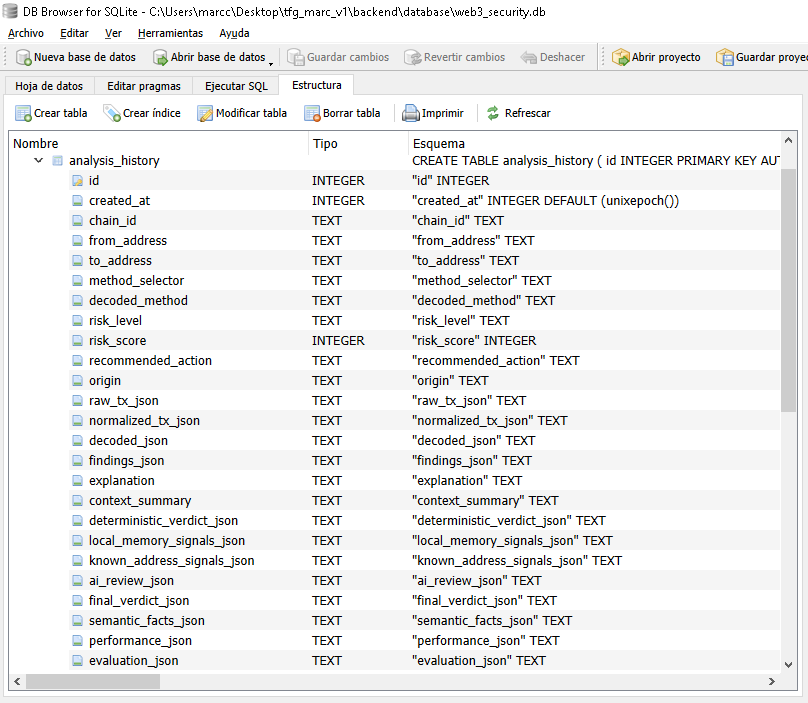
\includegraphics[width=0.88\textwidth]{imgs/sqlite_analysis_history_schema.png}
    \caption{Estructura de la taula \texttt{analysis\_history} a la base de dades SQLite local}
    \label{fig:sqlite-schema}
\end{figure}

\begin{figure}[p]
    \centering
    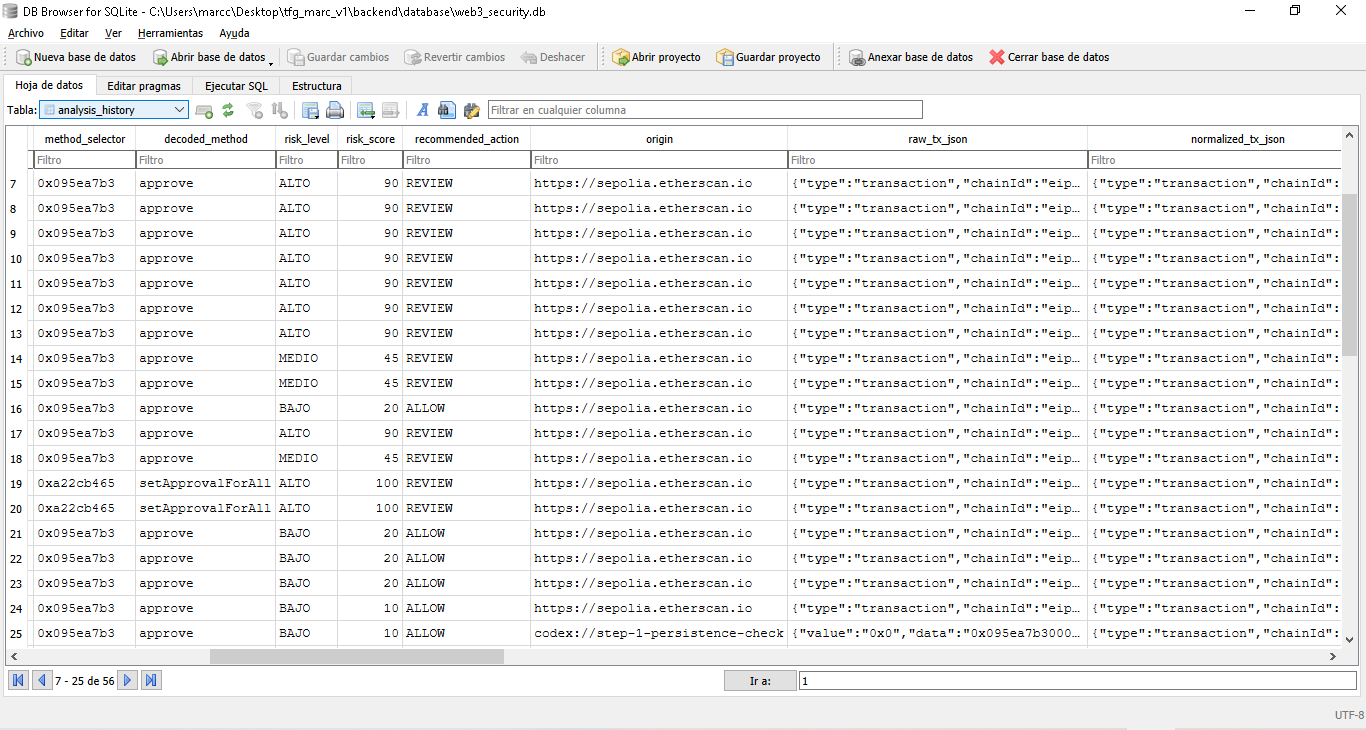
\includegraphics[width=\textwidth]{imgs/sqlite_analysis_history_rows.png}
    \caption{Registres d’anàlisi persistits a la base de dades SQLite local}
    \label{fig:sqlite-records}
\end{figure}


\subsubsection{Fonts externes de context i adreces conegudes}

A més de l’historial generat pel mateix sistema, el \textit{backend} pot utilitzar informació procedent de fonts externes per aportar context sobre les adreces que intervenen en una transacció. Aquesta funcionalitat té com a objectiu complementar l’anàlisi determinista amb etiquetes prèviament associades a adreces conegudes, com ara contractes legítims, adreces sospitoses o adreces relacionades amb activitats malicioses.

En la implementació actual s’ha incorporat informació procedent del repositori públic \textit{ethereum-lists}, mantingut per MyEtherWallet \cite{mew_ethereum_lists}. Concretament, s’utilitzen les llistes \texttt{addresses-darklist.json} i \texttt{addresses-lightlist.json}, que contenen adreces etiquetades amb informació de reputació. La primera agrupa principalment adreces relacionades amb estafes, \textit{phishing} o altres comportaments potencialment maliciosos, mentre que la segona permet identificar adreces conegudes o considerades legítimes dins de l’ecosistema Ethereum.

La importació d’aquestes dades es realitza mitjançant l’\textit{script}:

\begin{center}
\texttt{backend/scripts/import\_mew\_ethereum\_lists.js}
\end{center}

Aquest procés transforma la informació de les llistes externes i l’emmagatzema a la taula local \texttt{known\_addresses} de la base de dades SQLite. D’aquesta manera, el sistema no necessita consultar el servei extern durant cada anàlisi, sinó que pot treballar amb una còpia local de les dades importades. Aquest plantejament redueix la dependència de serveis remots, facilita la reproducció de les proves i manté la consulta de reputació dins de l’entorn local.

Durant l’anàlisi d’una transacció, el \textit{backend} comprova les adreces més rellevants de l’operació. Aquestes poden incloure l’adreça de destinació de la transacció, el camp \textit{spender} d’una aprovació ERC20 o l’\textit{operator} d’un permís global ERC721. Quan alguna d’aquestes adreces coincideix amb un registre de \texttt{known\_addresses}, el sistema incorpora la categoria, la descripció i la font de l’etiqueta al context de l’anàlisi.

La influència d’aquesta informació depèn del tipus d’etiqueta detectada. Una coincidència amb una adreça catalogada com a maliciosa, fraudulenta o inclosa en una llista negra pot generar un \textit{finding} específic i elevar el nivell de risc del veredicte. Les etiquetes de tipus advertiment o sospita aporten una senyal de cautela, mentre que les adreces conegudes, de confiança o associades als contractes de prova poden proporcionar context positiu sense anul·lar altres riscos detectats.

En qualsevol cas, la reputació externa no substitueix el motor de regles deterministes. Una etiqueta constitueix una font addicional de context, però no es considera per si sola una prova absoluta sobre la seguretat o perillositat d’una transacció. El veredicte final continua tenint en compte el tipus d’operació, els permisos concedits, els patrons detectats i la resta d’informació disponible.

Aquesta separació permet combinar criteris explícits i reproduïbles amb informació contextual actualitzable. En futures versions, el mateix mecanisme podria ampliar-se amb noves fonts públiques de reputació sense modificar el Snap ni la resta del flux principal del sistema.

La Figura~\ref{fig:known-addresses-dashboard} mostra la consulta d’aquest conjunt des del quadre de comandament. La interfície permet cercar i filtrar les adreces, i identifica tant les entrades manuals com les importades de fonts externes mitjançant la seva etiqueta, el tipus i la procedència.

\begin{figure}[H]
    \centering
    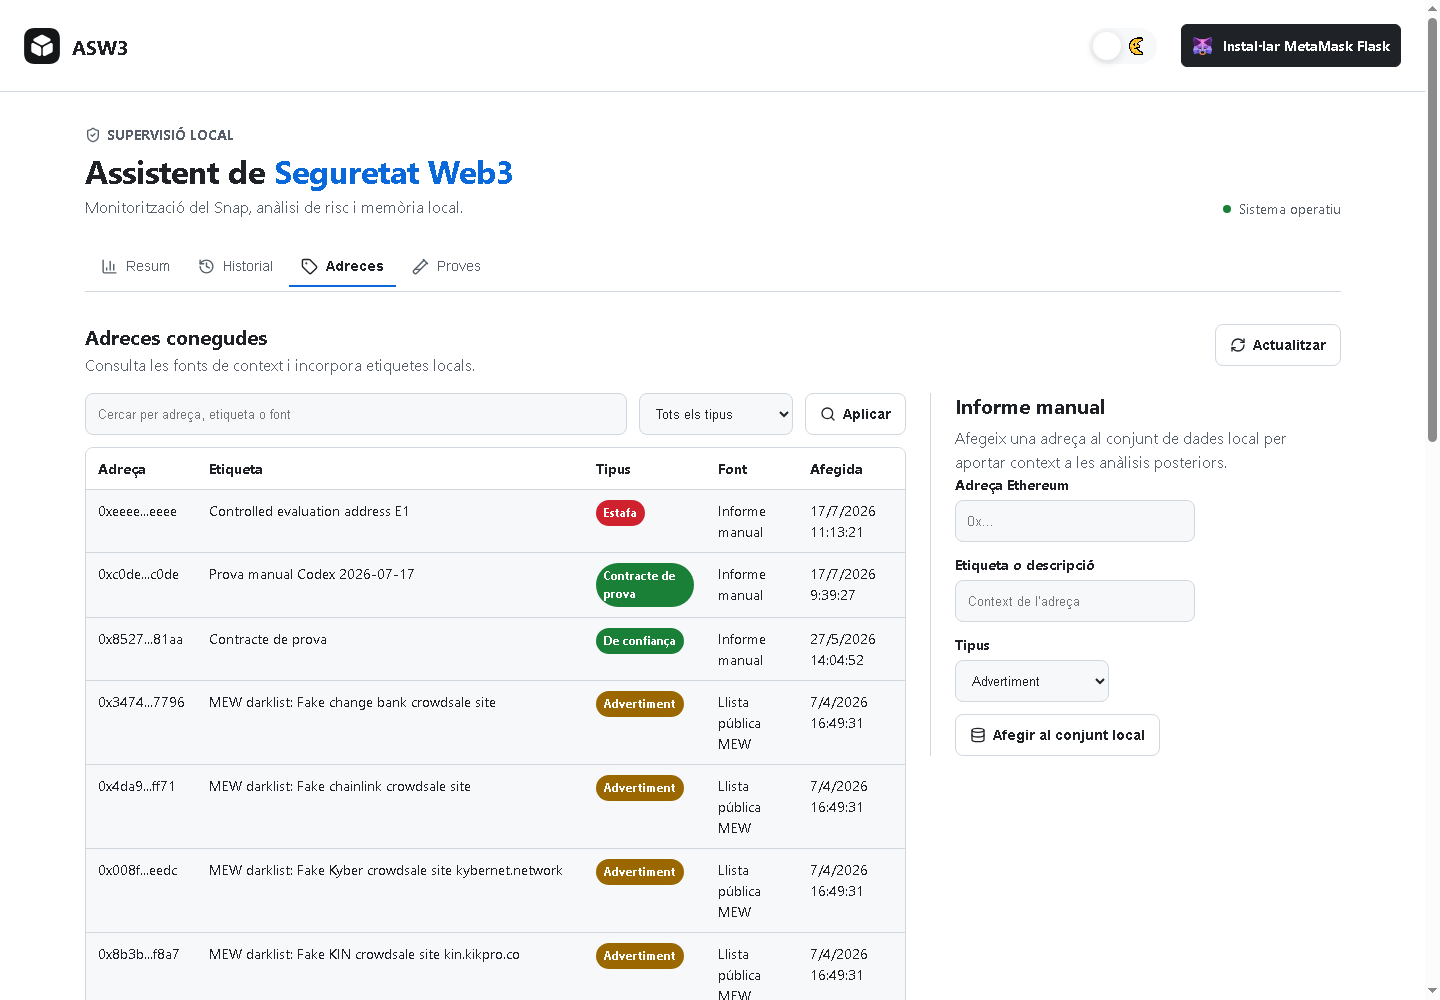
\includegraphics[width=\textwidth]{imgs/known_addresses_dashboard.png}
    \caption{Consulta i filtratge del conjunt local d’adreces conegudes}
    \label{fig:known-addresses-dashboard}
\end{figure}


\subsubsection{Construcció de la resposta}

Després de completar el procés d’anàlisi, el backend construeix una resposta estructurada en format JSON que s’envia novament al Snap. En les primeres versions del prototip, aquesta resposta contenia principalment dos camps: el nivell de risc i l’explicació generada. Amb l’evolució del sistema, però, l’estructura s’ha ampliat per incorporar més informació contextual i fer el resultat més complet i traçable.

En la versió actual, la resposta inclou el veredicte final de risc, l’acció recomanada, la puntuació associada, els indicis detectats en el camp \texttt{findings}, la informació procedent de la memòria local i les coincidències amb adreces conegudes. També pot incorporar la revisió complementària generada per la IA mitjançant l’objecte \texttt{ai\_review}, que conté camps com el nivell de risc suggerit, la confiança, els indicadors textuals detectats i un resum justificatiu.

El contingut textual generat a partir d’aquesta versió s’expressa en català, inclosos els indicis, els motius del veredicte, els missatges d’error i les explicacions deterministes o assistides per Ollama. En canvi, els noms dels camps i els valors enumerats de risc i acció es mantenen estables per compatibilitat. La traducció d’aquests valors es realitza exclusivament a la capa de presentació de la DApp i del Snap.

El veredicte final es construeix combinant el resultat determinista amb la revisió complementària de la IA. Les regles deterministes mantenen la prioritat en els patrons de risc clarament identificats, mentre que la IA només pot aportar context addicional o elevar el nivell de cautela en determinats casos. D’aquesta manera, el model de llenguatge no pot reduir un risc detectat prèviament pel motor de regles.

Abans d’incorporar l’explicació i la revisió de la IA a la resposta definitiva, el backend aplica una capa de control semàntic. Aquesta capa comprova que les afirmacions generades siguin compatibles amb els fets detectats durant l’anàlisi, com ara l’existència d’una aprovació il·limitada, un permís global, una revocació, un enviament de valor o una coincidència amb una adreça etiquetada. Quan la resposta generada és buida, massa extensa o conté contradiccions, el sistema la substitueix per una explicació segura construïda de manera determinista.

La resposta final pot contenir, entre altres elements, els camps següents:

\begin{itemize}
    \item el veredicte final i el nivell de risc;
    \item la puntuació de risc;
    \item l’acció recomanada;
    \item els indicis principals del camp \texttt{findings};
    \item el context procedent de la memòria local;
    \item les coincidències amb adreces conegudes;
    \item la revisió complementària de la IA;
    \item l’explicació final mostrada a l’usuari;
    \item les metadades bàsiques de la transacció, com la xarxa o l’origen;
    \item l'identificador persistent \texttt{analysis\_id}, les mesures de rendiment i, quan correspon, les metadades d'avaluació.
\end{itemize}

Aquesta resposta ampliada permet mantenir el Snap com un component lleuger. El Snap no necessita reconstruir el raonament intern del backend ni aplicar les regles de risc, sinó que es limita a adaptar la informació rebuda al format visual permès per MetaMask Snaps. D’aquesta manera, el backend conserva la responsabilitat de l’anàlisi i el Snap se centra en la presentació del resultat dins de la interfície de confirmació.

La Figura~\ref{fig:backend-pipeline} sintetitza el flux intern complet del \textit{backend}, des de la recepció i normalització de la petició fins a la construcció de la resposta que es retorna al Snap. El diagrama mostra la intervenció dels principals mòduls d’anàlisi, persistència, context i generació d’explicacions.

\begin{figure}[htbp]
    \centering
    \colorbox{white}{%
        
\includegraphics[width=\dimexpr\textwidth-2\fboxsep\relax]{imgs/impl_backend.png}%
    }
    \caption{\textit{Pipeline} intern del \textit{backend} d’anàlisi}
    \label{fig:backend-pipeline}
\end{figure}
